\subsection{The Challenges: Foregrounds and Systematics}
\label{sec:foregrounds}
\vspace{-0.05in}

%A satellite mission provides a unique opportunity to target both the inflationary B-mode polarization that originates from the epoch of recombination and peaks around $\ell=80$ and the contribution that peaks on significantly larger scales $\ell\lesssim 12$. To measure the contribution from reionization will require an unprecedented understanding of foregrounds and systematic effects. This is illustrated in the left panel of Figure~\ref{fig:Qrp001}, which shows the contribution from reionization to the Stokes $Q$-parameter for $r=0.001$. The amplitude of the signal is approximately $10$ nK

The search for primordial $B$-modes is one of the main science
objectives of future CMB missions. A satellite experiment enables
full-sky observations, and provides complete flexibility in the choice
of frequency coverage, both of which are challenging from the ground
or from the balloon platform.  Among other limitations, the atmosphere
prevents observations at key frequencies, such as 60\,GHz, and
requires data filtering that makes it difficult to recover the larger
angular scales.

By the time a probe-class mission launches, substantial progress will
have been made in this quest.  In the absence of a primordial $B$-mode
signal at detectable levels, the mission will significantly improve
the upper limit on the tensor-to-scalar ratio $r$, with
$\sigma(r)\!\sim\!10^{-3}$.  However, if $r$ is large enough,
tentative $B$-mode detections could be reported from the ground or by
ballon experiments ahead of this mission. The significance of such a
discovery would be such that the detailed characterization of the
angular and spectral dependence of the signal, as well as the
verification of its isotropy across the sky, both of which are
uniquely enabled by a satellite mission, would be required to confirm
its primordial origin \comred{(cite Decadal Survey)}.

In this scenario, a probe-class mission will in particular detect and
characterize the reionization signal expected at the largest angular
scales (multipoles below $\sim\!10$), where observations from other
platforms are the most challenging. The contribution from reionization
to the Stokes parameter $Q$ for $r=0.001$ is shown in the left panel
of Figure~\ref{fig:Qrp001}. The amplitude of this signal is
$\sim\!10$\,nK, which requires that any experiment attempting to
measure it control large-scale foregrounds and systematics at the
unprecedented level of a few nK.

\begin{figure}[h]
\begin{center}
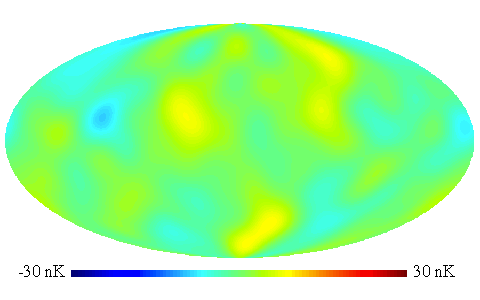
\includegraphics[width=3.2in]{Figures/P15_2_12_rp001.pdf}
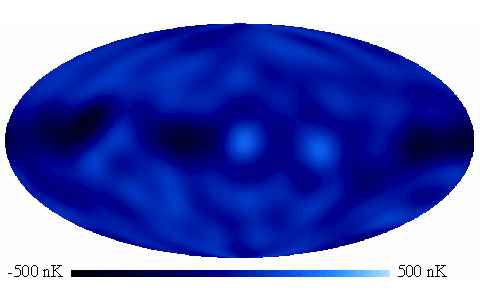
\includegraphics[width=3.2in]{Figures/P353_N_2_12.pdf}
\end{center}
\caption{{\it Left panel:} Contribution to the Stokes $Q$ parameter
  from inflationary $B$-modes for $\ell<12$ and $r=0.001$. {\it Right
    panel:} Noise in the $Planck$ 353 GHz map of the Stokes $Q$
  parameter for $\ell<12$ rescaled to 150\,GHz assuming the spectral
  properties of dust.}
\label{fig:Qrp001}
\end{figure}

\subsubsection{Foregrounds}

Data from the \emph{Planck} satellite have significantly improved our
understanding of foregrounds in both intensity and polarization.
 %In intensity, $Planck$, for example, showed the unexpected relevance of Carbon-Monoxide lines at moderate latitudes as well as the existence of an anomalous emission from dust at low frequencies.
In polarization, the sky is dominated by the expected sources, namely
synchrotron and dust emission. \emph{Planck} has provided us with much
improved measurements of their amplitude and spectral dependence. The
observed frequency spectra of both foregrounds are shown for three sky
fractions in the left panel of Figure~\ref{fig:frequency}.  \emph{Even
  in the cleanest patches of the sky}, polarized foreground emission
is brighter than the sought-after primordial $B$-mode signal by over
an order of magnitude at all frequencies.  This statement holds at all
angular scales relevant to the search for primordial $B$-modes, as
shown in the right panel of Figure~\ref{fig:frequency}.

Perfect knowledge of the foreground components would enable their
removal from microwave data, but the sensitivity of the \emph{Planck}
measurements limits it at a level insufficient to detect primordial
$B$-modes, even for values of $r\!\sim\!10^{-1}$. The right panel of
Figure~\ref{fig:Qrp001} shows the noise in the \emph{Planck} 353\,GHz
map of the Stokes $Q$ parameter at the angular scales relevant for
primordial $B$-mode measurements, and rescaled to 150\,GHz assuming
the spectral dependence of dust; it is over an order of magnitude
larger than the inflationary contribution for $r=0.001$.  A mission
aiming to detect primordial $B$-modes at this level across the sky
will therefore not be able to rely on existing data. High
signal-to-noise foreground measurements must accompany those at
frequencies where the CMB contribution is larger.  As discussed below,
optimizing the frequency coverage of these measurements will be a key
goal of the mission concept study.

While the search for primordial B-modes leads to the strictest constraints on foreground residuals, exquisit control of foregrounds is also necessary for other science objectives. A satellite mission is likely also the only reliable way to measure the optical depth at a level necessary to break the degeneracy with the neutrino mass. Furthermore, a cosmic variance limited measurement of E-mode polarization on large scales possible with a probe mission would contain valuable information about the star formation history. 

Similarly, a clear objective of the spectral science is to have a robust, foreground-marginalized expectation of detecting the $\mu$-distortion generated by the dissipation of small-scale acoustic modes in $\Lambda$CDM. While an instrument like PIXIE just falls short of this objective, it seems within reach of a probe mission.

\begin{figure}[h]
\begin{center}
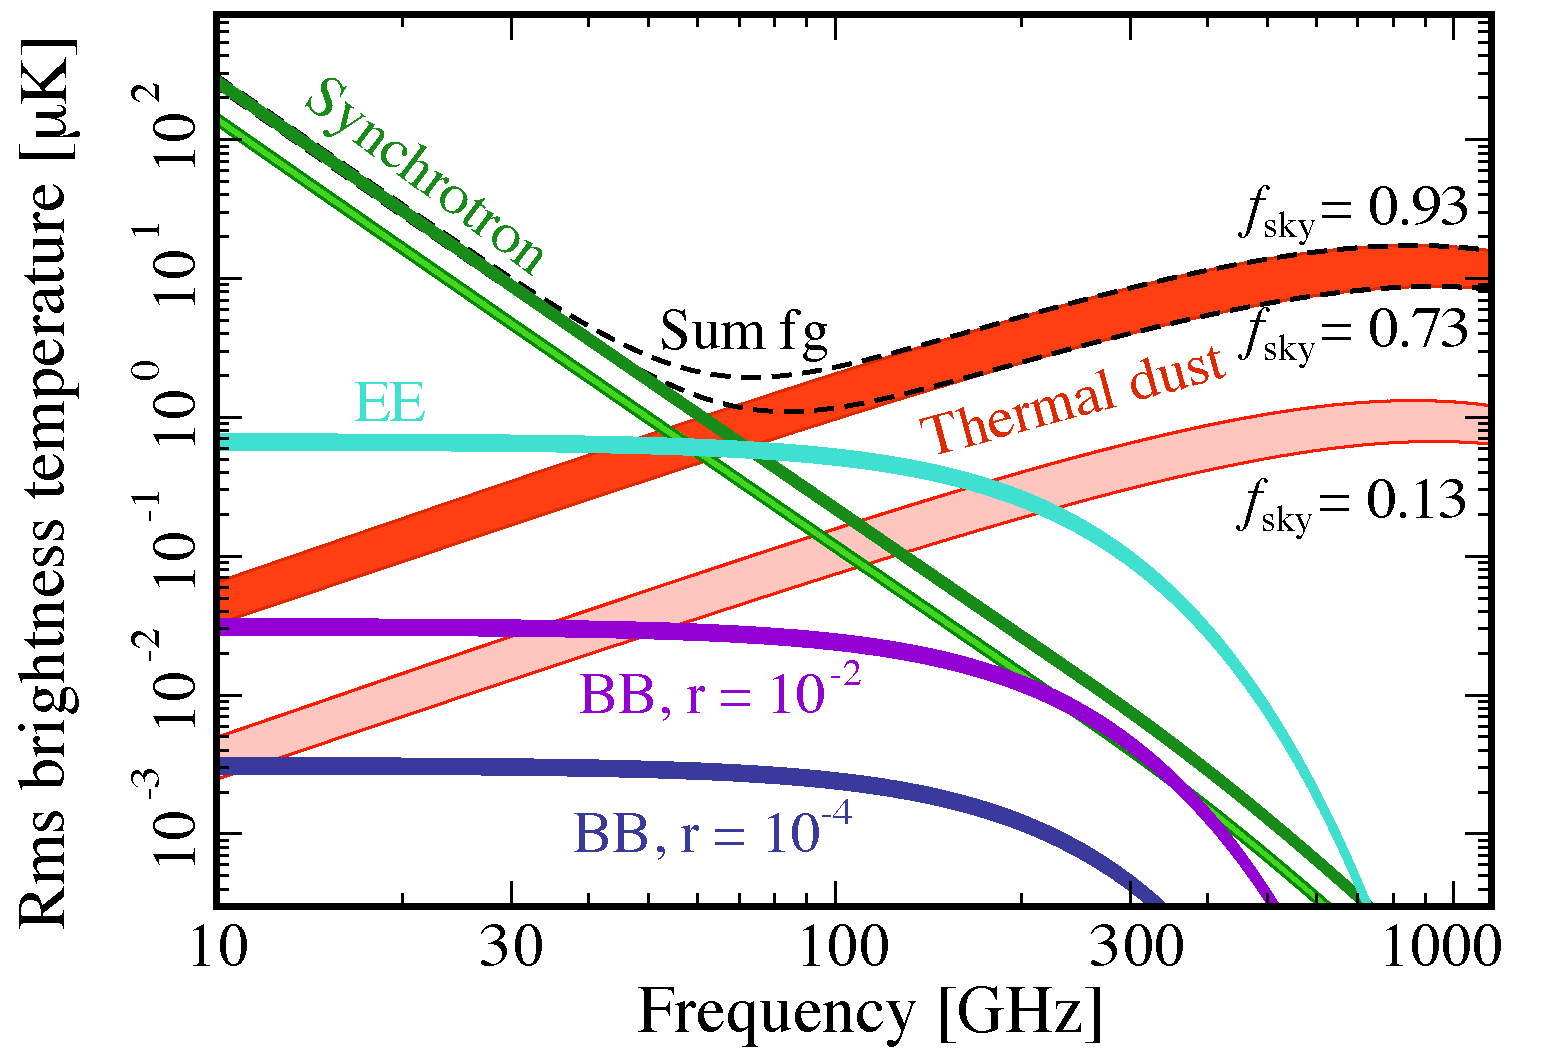
\includegraphics[width=3.26in]{Figures/overview_pol_v4_fsky_noplanck.pdf}\hskip .2cm
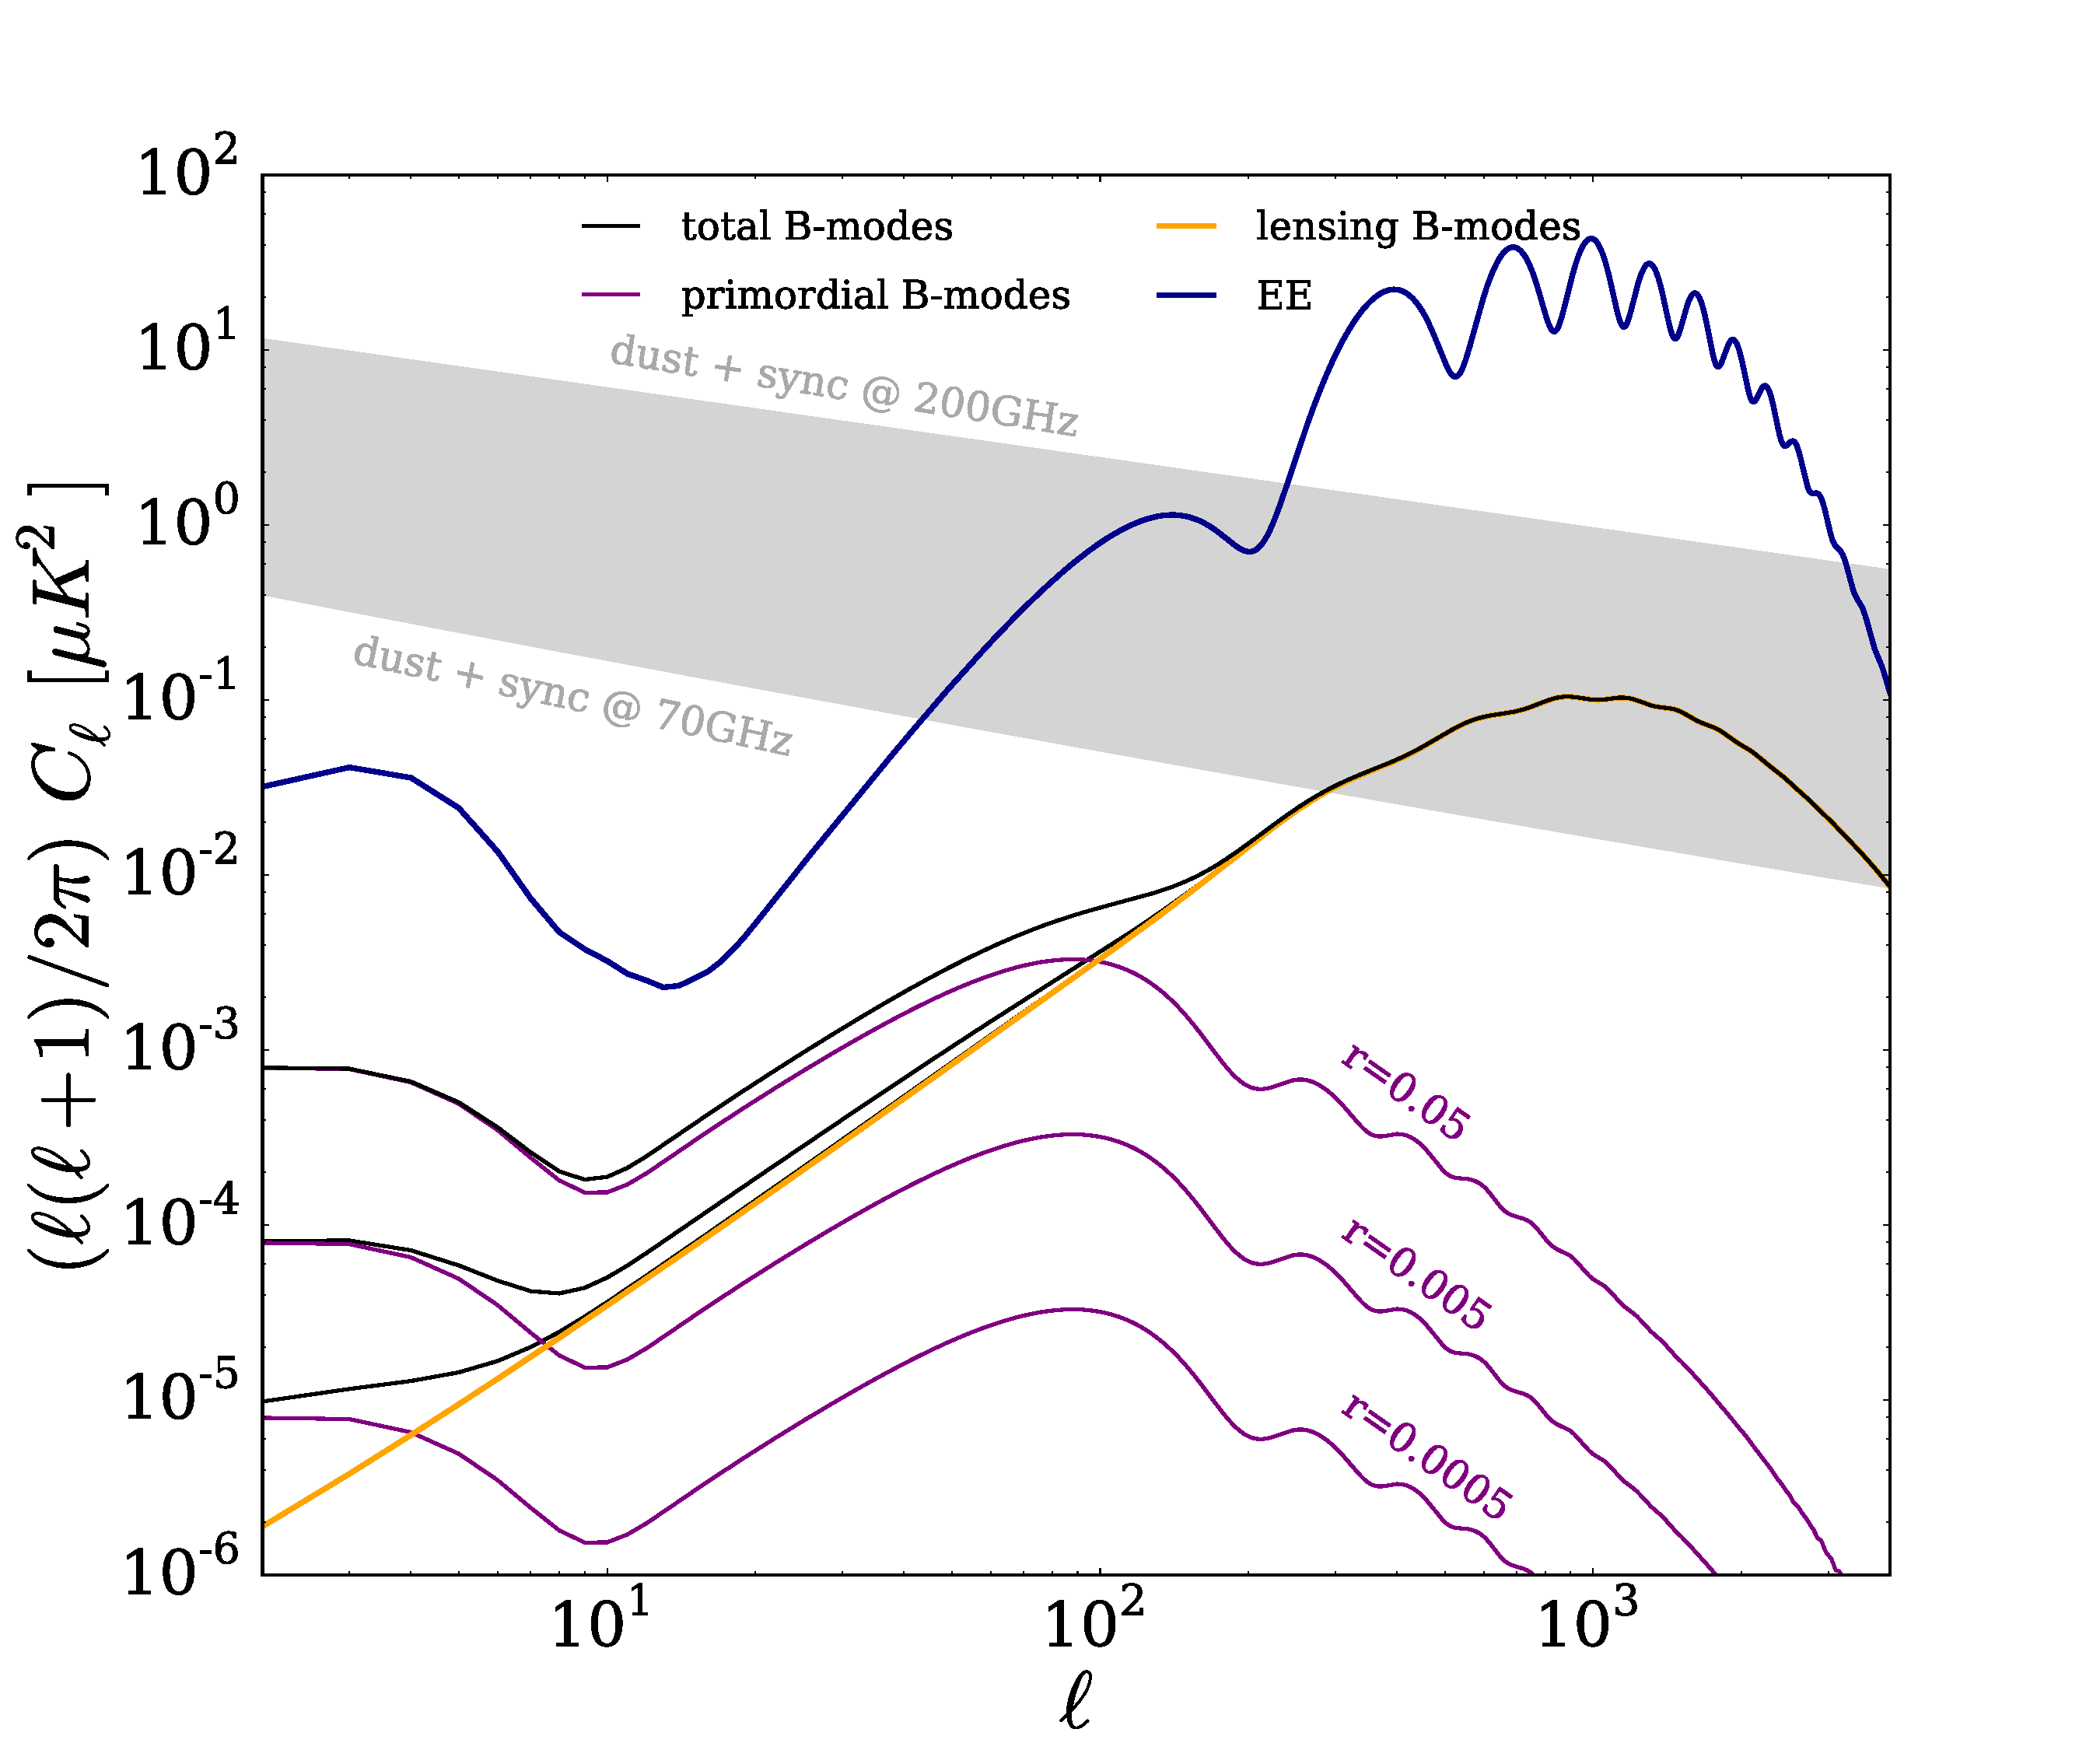
\includegraphics[width=3.12in]{Figures/clbb_freq_v2.pdf}
\end{center}
\caption{{\it Left panel:} Brightness temperature as function of frequency for the CMB as well as synchrotron emission (green) and dust emission (red). The darker bands show the brightness temperature for sky fractions between $73\%$ and $93\%$, the lighter bands show the brightness temperature for the cleanest $13\%$ with the width indicating the uncertainty. {\it Right panel:} Angular power spectrum for B-mode polarization of the CMB for $r=0.0005$, $r=0.005$, and $r=0.05$ as well as for foreground emission between 70 and 200 GHz.}
%, which shows the power spectrum of
%foregrounds over $75\%$ of the sky for frequencies between $70$ and
%$200$ GHz together with the lensing and inflationary contribution for
%different values of the tensor-to-scalar ratio.
\label{fig:frequency}
\end{figure}


One of the key ingredients in the design of a CMB experiment is the frequency coverage required to achieve the science goals. Consequently, optimizing frequency coverage in light of the new information from $Planck$ and its limitations will be one of key task of the study proposed here.   

To achieve these goals we plan to investigate the effect on the measurements of r and $\tau$ of the presence of foregrounds residuals in the CMB maps (after foreground separation and/or cleaning) including, for example, the properties of the polarized thermal dust emission, specifically the potential spatial variation of its spectral index, hinted at by the observed decorrelation of the dust between 217 GHz and 353GHz Planck channels (\ref{Planck2015-X;Planck2015-L;Planck2015-XXIX;Boulanger2016}), and the study of the breakdown of the modified black body spectrum model. 
These aspects are better explored with the help of physically motivated models of the foregrounds (\ref{Bruce+Fraisse2009,Hensley et al in preparation}) and simulations based on these, using either existing simulation tools and/or implementing new simulators when required. 

The optimization of frequency channels will be conducted using both traditional (Fisher codes both spectra and map based) and novel techniques currently in development (such as direct Bayesian MCMC inference of cosmological parameters in the presence of foregrounds, (extension of the method presented in  \ref{Jewell2016}). Realistic simulations (including time domain based) are essential to fully assess the performance of a given instrument design/concept in view of both foreground residuals and the presence of systematics. We plan to generate these simulations, process them as we would do the real data, specifically applying some of the current component separation methods to clean the frequency maps from foreground emission (akin to {\it Planck} collaboration procedures \ref{Planck2015-IX}) and propagate to parameter estimation, assessing the impact of all contaminating effects on the accuracy and potential biases of the parameters estimated with particular emphasis on r and $\tau$.



%references
%Bruce+Fraisse2009 - 2009ApJ...696....1D
%Planck2015-IX - 2016A&A...594A...9P
%Planck2015-X - 2016A&A...594A..10P
%Planck2015-XXIX - A&A 586, A132 (2016)
%Planck2015-L - arXiv:1606.07335v1;
%Boulanger2016 - A&A 580, A136 (2015)
%Jewell2016 -  ApJ., 820, 2016
%





% Raphael, Josquin, Aurelien, Charles, Graca
